\RequirePackage{amsmath}
\documentclass{llncs}

\usepackage{cmap}
\usepackage[utf8]{inputenc}
\usepackage[T2A]{fontenc}

\usepackage{tikz}

\usepackage[font=small]{caption}
\usepackage{subcaption}

\usepackage{hyperref}

\usepackage{listings}
\usepackage{xcolor}

\usepackage{xspace}

\tikzset{every picture/.append style={scale=0.5}}

\tikzstyle{cell}=[rectangle,draw=gray,dashed,thick, minimum size=1.05cm]
\tikzstyle{graybox}=[rectangle,thick, minimum size=0.4cm, fill=lightgray]
\tikzstyle{whitebox}=[rectangle,draw=black,thick, minimum size=0.5cm]

\lstset{
  language=c++,
  basicstyle=\ttfamily \scriptsize,
  lineskip={-1.5pt},
  columns=fixed,
  basewidth=0.5em,
  keywordstyle=\bfseries\color{blue!60!black},
  commentstyle=\itshape\color{gray!80!black},
  identifierstyle=\color{violet!60!black},
  stringstyle=\color{orange},
  frame=single
  % numbers=left
}

\newcommand{\norm}[1]{\left\lVert#1\right\rVert}
\renewcommand{\C}{\texttt{C}\xspace}

\begin{document}

\title{Optimization for connected-component counting in binary image for the case of
8-connectivity}

\author{Fedor Alekseev\inst{1} \and Mikhail Alekseev\inst{2}\inst{3}
\and Artyom Makovetskii\inst{2}\inst{4}}

\institute{Moscow Institute of Physics and Technology State University, Dolgoprudny, Russia\\
\email{alekseev@phystech.edu}
\and
Chelyabinsk State University, Chelyabinsk, Russia
\and
\email{alexeev@csu.ru}
\and
\email{artemmac@mail.ru}}

\maketitle              % typeset the title of the contribution

\begin{abstract}
The linear variation is a topological characteristic of the function of two variables.
The problem of linear variation computing can be reduced to the problem
of counting connected components in a binary image with eight-connected connectivity.
The new hybrid method for the problem is presented.
The method is essentially a modification of a two-scan algorithm for labeling
that groups the pixels into $2 \times 2$ cells.

\keywords{Binary raster image, connected component labeling,
pattern recognition}
\end{abstract}

\section{Introduction}

% Makovetskii part

In image restoration it is often necessary to consider the following problem.
How to restore an original undistorted image $v$, if it is known an observed
image $u_0$ and the relation between $u_0$ and $v$:
\begin{equation}
  u_0=v+n,
  \label{eq:imageRelation}
\end{equation}
where $n$ is a noise?
A common way for solving the problems \ref{eq:imageRelation} is to use the
variational functionals.
One of the most widely used approaches is total variation 
regularization [1]. % TODO fix bibliography
Let $J(u)$ be the following functional:
\begin{equation}
  J(u) = \frac12 \norm{u - u_0}^2 + \lambda TV(u),
  \label{eq:jFunctional}
\end{equation}
where $\norm{\cdot}$ is the $L_2$ norm and all function we consider belong to the class
$BV(\Omega)$, i.\,e. the class of bounded variation on the set $\Omega$ functions.
%
The expression $\frac12 \norm{n-n_0}^2$ is called a fidelity term and
$\lambda TV(u)$ is called a regularization term and $\lambda$ is regularization
parameter.

% Alekseev part

This problem is equivalent to the problem of counting the number of connected
components (CC) in a binary image with 8-connectivity.
This is usually done through CC labeling, and many approaches for that are
known\cite{sterzh}.

This paper presents an efficient way to convert the initial binary image
with 8-connectivity into
a condensed (non-binary) image with new connectivity that is $2$ times smaller in
each dimension than the initial image.
Most approaches for CC labeling are still valid for the new matrix.
As time and memory consumptions of conventional approaches usually depend linearly on
the number of pixels, running them on the condensed image can be up to 4 times
more efficient than running on the initial image.

It is worth noting that our method exploits an important property of 8-connectivity
that does not hold for 4-connectivity, so it is not applicable for the latter case.

\section{$2\times2$ condensation}

We will use the fact that for the case of 8-connectivity all $4$ pixels of any
$2 \times 2$ square are adjacent to each other, and so are contained in the same CC
and should have same labels upon completion of the labeling algorithm.
So instead of labeling single pixels we can label $2 \times 2$ groups of pixels,
or ``cells''.

Consider a $2N \times 2M$ binary image\footnote{
For convenience in this paper we consider only input images with even size
in both dimensions. If this is not the case, one can easily append a row or
a column of background pixels to the image.}
specified by a binary predicate $b(x, y)$,
returning $1$ in case the pixel at the given coordinates is black (object pixel),
and $0$ otherwise (background pixel).
For convenience we use 0-indexation throughout the paper, so the topmost row has
row index $y=0$, and the leftmost column has column index $x=0$.

The condensed image will be of size $N \times M$.
Each pixel of the condensed image will unambiguously represent the configuration
of the corresponding $2\times 2$ cell of pixels of the initial binary image.
So the condensed image will contain pixels of $2^4 = 16$ colors.
We suggest the function $c(x, y)$ denoting the color of a pixel of condensed image
to be the following:
\begin{align*}
  c(x, y) &= 2^0 b(2x, 2y)   + 2^1 b(2x+1, 2y) \\
          &+ {} 2^2 b(2x, 2y+1) + 2^3 b(2x+1,2y+1)
\end{align*}

So the value of each pixel of the initial image is stored in the corresponding
bit in color of the corresponding pixel of the condensed image.
Note that if $c(x, y) = 0$ for some $(x, y)$, then there are no object pixels in
this cell, and no label should be assigned to this whole cell. The enumeration of
pixels inside one cell is shown on \autoref{fig:pixelsEnumeration}.

\begin{figure}[t]
  \centering
  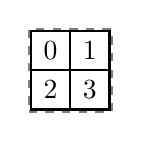
\begin{tikzpicture}
    \node[cell] at (0.5, 0.5) {};
    \foreach \x/\y [count=\i from 0] in {0/1,1/1,0/0,1/0} {
      \node[whitebox] at (\x,\y) {\i};
    }
  \end{tikzpicture}
  \caption{Cell pixels enumeration}
  \label{fig:pixelsEnumeration}
\end{figure}

We need also to define connectivity function for the condensed image.
We cannot actually just use 8-connectivity, as whether two cells are adjacent
cells of one CC depends not only on their coordinates, but also on their
configuration. See \autoref{fig:connectivity:examples} for examples.

\begin{figure}
  \centering
  \begin{subfigure}[t]{0.3\linewidth}
    \centering
    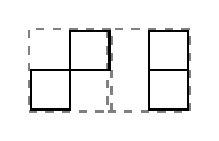
\begin{tikzpicture}
      \foreach \x in {0.5,2.5}
        \node[cell] at (\x,0.5){};
      \foreach \x/\y in {0/0, 1/1, 3/0, 3/1}
        \node[whitebox] at (\x, \y){};
    \end{tikzpicture}
    \caption{Nearby cells that are not directly connected.}
  \end{subfigure}
  \quad
  \begin{subfigure}[t]{0.3\linewidth}
    \centering
    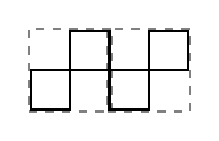
\begin{tikzpicture}
      \foreach \x in {0.5,2.5}
        \node[cell] at (\x,0.5){};
      \foreach \x/\y in {0/0, 1/1, 2/0, 3/1}
        \node[whitebox] at (\x, \y){};
    \end{tikzpicture}
    \caption{Directly connected cells.}
  \end{subfigure}
  \quad
  \begin{subfigure}[t]{0.3\linewidth}
    \centering
    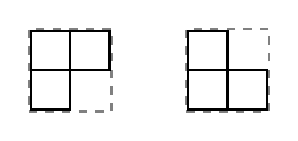
\begin{tikzpicture}
      \foreach \x in {0.5,4.5}
        \node[cell] at (\x,0.5){};
      \foreach \x/\y in {0/0, 0/1, 1/1, 4/0, 4/1, 5/0}
        \node[whitebox] at (\x, \y){};
    \end{tikzpicture}
    \caption{Cells that are not nearby in terms of 8-connectivity, cannot be
    directly connected.}
  \end{subfigure}
  \caption{Cells connectivity examples}
  \label{fig:connectivity:examples}.
\end{figure}

However, for every variant of relative placement of two nearby cells there is
a mask of pixels of each cells that are important for direct connectivity of
this pair of cells.
So two cells are considered directly connected, if they are nearby
in terms of 8-connectivity and each of them contains at least one object pixel
in the mask of important pixels corresponding to relative placement of the cells.
The masks are shown in \autoref{fig:connectivity:masks}.

\begin{figure}
  \centering
  \begin{subfigure}[t]{0.2\linewidth}
    \centering
    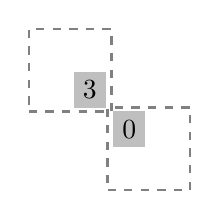
\begin{tikzpicture}
      \node[cell] at (0.5, 2.5) {};
      \node[cell] at (2.5, 0.5) {};
      \node[graybox] at (1, 2) {3};
      \node[graybox] at (2, 1) {0};
    \end{tikzpicture}
  \end{subfigure}
  \begin{subfigure}[t]{0.2\linewidth}
    \centering
    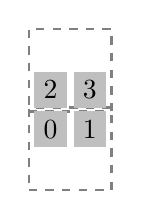
\begin{tikzpicture}
      \node[cell] at (0.5, 2.5) {};
      \node[cell] at (0.5, 0.5) {};
      \node[graybox] at (0, 2) {2};
      \node[graybox] at (1, 2) {3};
      \node[graybox] at (0, 1) {0};
      \node[graybox] at (1, 1) {1};
    \end{tikzpicture}
  \end{subfigure}
  \begin{subfigure}[t]{0.2\linewidth}
    \centering
    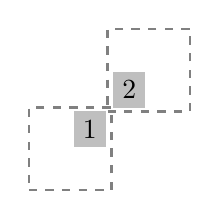
\begin{tikzpicture}
      \node[cell] at (0.5, 0.5) {};
      \node[cell] at (2.5, 2.5) {};
      \node[graybox] at (1, 1) {1};
      \node[graybox] at (2, 2) {2};
    \end{tikzpicture}
  \end{subfigure}
  \begin{subfigure}[t]{0.25\linewidth}
    \centering
    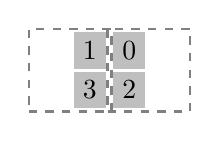
\begin{tikzpicture}
      \node[cell] at (0.5, 0.5) {};
      \node[cell] at (2.5, 0.5) {};
      \node[graybox] at (1, 0) {3};
      \node[graybox] at (1, 1) {1};
      \node[graybox] at (2, 0) {2};
      \node[graybox] at (2, 1) {0};
    \end{tikzpicture}
  \end{subfigure}
  \caption{Masks of important pixels for all four cases of relative placement
  of two nearby cells. Those pixels are filled in gray, with their numbers within
  cell specified.}
  \label{fig:connectivity:masks}
\end{figure}

The idea is that if we naturally encode mask pixels as 4-bit numbers in the
way similar to how we defined $c$, we can express the predicate denoting whether
two nearby cells
are directly connected efficiently with just two bitwise and one logical AND
operations.
As an example, \autoref{fig:connectivity:code} compares possible codes in \C checking
if the labels of the current pixel or cell and the one right on top of it
should be same for classic 8-connectivity and for the new connectivity.
Note that as bitwise operations are usually relatively cheap, we added only a
little complication compared to decreasing the number of pixels to process by the 
factor of 4.

\begin{figure}
  \centering
  \begin{subfigure}[t]{0.475\linewidth}
    \centering
    \begin{lstlisting}
    if (b(x, y)) {
      if (b(x, y-1)) {
        // copy labels, or union label sets
      }
      // consider other directions
    }
    \end{lstlisting}
    \caption{Binary image with 8-connectivity.}
  \end{subfigure}
  \quad
  \begin{subfigure}[t]{0.475\linewidth}
    \centering
    \begin{lstlisting}
    if (c(x, y)) {
      if ((c(x, y-1) & ((1<<2) | (1<<3)))
       && (c(x, y)   & ((1<<0) | (1<<1)))) {
        // copy labels, or union label sets
      }
      // consider other directions
    }
    \end{lstlisting}
    \caption{Condensed image with new connectivity.}
  \end{subfigure}
  \caption{Checking the nearby top pixel/cell.}
  \label{fig:connectivity:code}
\end{figure}

\section{Benchmarks}

\begin{thebibliography}{5}

\bibitem {hechao}
He, L., Chao, Y., Suzuki, K., Wu, K.:
Fast connected-component labeling. Pattern Recognition. v42, Pages 1977-1987. (2009)

\bibitem {sterzh}
Стержанов, М.:
Методики выделения связных компонент в штриховых бинарных изображениях.
Труды конференции ГрафиКон’2010. НИУ ИТМО. Санкт-Петербург. 2010, с. 169-174.

\end{thebibliography}

\end{document}
